\begin{figure}[ht]
    \centering

    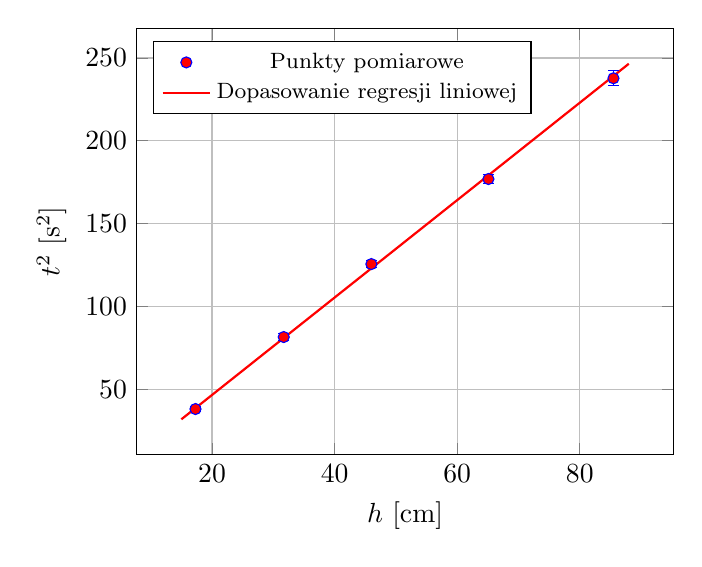
\begin{tikzpicture}
        \begin{axis}[
            width=8.4cm, height=7cm,
            xlabel={$h~[\mathrm{cm}]$},
            ylabel={$t^2~[\mathrm{s}^2]$},
            legend pos=north west,
            grid=major,
            legend style={font=\footnotesize}
        ]

        \addlegendimage{only marks, mark=*, blue, mark options={fill=red}, error bars/.cd, y dir=both, y explicit}
        \addlegendentry{Punkty pomiarowe}
        
        \addlegendimage{no markers, red, thick}
        \addlegendentry{Dopasowanie regresji liniowej}
        
        \def\slope{2.9411189}
        \def\intercept{-12.32102}
        
        \addplot [red, thick, domain=15:88, forget plot] {\slope*x + \intercept};
        \addlegendentry{Dopasowanie regresji liniowej}
    
        \addplot+[
            only marks,
            mark=*,
            blue,
            mark options={fill=red},
            forget plot,
            error bars/.cd,
            y dir=both,
            y explicit,
        ] table [x=x, y=y, y error=err] {
            x       y               err
            17.3    38.00106025     1.22030149
            31.7    81.47048121     1.924432727
            46.0    125.5408203     2.062786691
            65.1    176.9033003     2.683325469
            85.5    237.745561      4.544923276
        };
        \addlegendentry{Punkty pomiarowe}
    
        \end{axis}
    \end{tikzpicture}

    \caption{
        Dane pomiarowe dla Zależności II wraz z dopasowaniem regresji liniowej: $t^2(h) = ah + b$. Niepewności $t^2$ są ledwo widoczne na wykresie, niepewności $h$ są na tyle małe, że nie widać ich wcale.}
    \label{img:regresja-i-wykres}
\end{figure}
